\chapter{Grundlagen}\label{ch:data}

\section{Definition von Datenqualität}
Datenqualität wird in der Literatur auf verschiedene Arten definiert. 
Viele Datenqualitätsstudien verwenden Korrektheit als einziges Datenqualitätsmerkmal. \cite{wang1996}
Datenqualität umfasst jedoch nicht nur die Korrektheit von Daten, sondern auch anderen Dimensionen. 
Ein Paper von Oliva, Zubcoff und Mazón zeigt den Einfluss von anderen Dimensionen, wie zb. Vollständigkeit auf die Erkennungsrate von Klassifikatoren \cite{espinosaoliva2011} Die Autoren schlagen vor den Aufbereitungsprozess und vor allem Datenqualität nicht nur auf die Korrektheit von Daten zu beziehen sondern auch auf die anderen Datenqualitätsdimensionen zu achten.

\subsection{Datenqualitätsdimensionen}
\label{subsec:dimensionen}
Die Dimensionen Richtigkeit, Vollständigkeit, Konsistenz und Aktualität werden in den meisten Veröffentlichungen genannt, allerdings gibt es keinen Standard, weder im Bezug auf die verwendeten Dimensionen, noch die Definition der Dimensionen. \cite{scannapieco2002}
Da keine allgemeine Empfehlung zur Verwendung von Dimensionen existiert werden in dieser Arbeit die Datenqualitätsdimensionen verwendet, die in den meisten Veröffentlichungen auftauchen.
Dies kann dem Paper von Scannapieco und Catarci entnommen werden. 
Diese Dimensionen sind für die Auswertung der Methoden im Rahmen der Arbeit geeignet. 
Jede dieser Datenqualitätsdimensionen umfasst eine Facette der Datenqualität und werden im Folgenden nach Wand und Wang beschrieben \cite{wand1996}. \\

\textbf{Richtigkeit} \\
Richtigkeit wird als Gleichheit zwischen zwei Werten definiert, sodass die Daten die Wirklichkeit korrekt repräsentieren. 
Beispiel: Eine Person mit dem Namen Max Mustermann ist als Mx Mustermann abgespeichert. 
Die gespeicherten Daten repräsentieren nicht die Wirklichkeit, sie sind somit nicht richtig. \\

\textbf{Aktualität / temporäre Richtigkeit} \\
Als Spezialisierung der Richtigkeit kann die temporäre Richtigkeit gesehen werden, die richtige Repräsentation zu einem bestimmten Zeitpunkt oder Zeitspanne beschreibt. 
Die temporäre Richtigkeit zum aktuellen Zeitpunkt wird auch als Aktualität bezeichnet. \\

\textbf{Vollständigkeit} \\
Die Daten sind umfangreich genug für die jeweilige Aufgabe. \cite{wang1996} 
Da ein Data Warehouse aus relationalen Datenbanken besteht, wird die Vollständigkeit im Folgenden auf relationale Datenbanken bezogen.
Die Vollständigkeit wird von \cite{pipino2002} in drei Klassen kategorisiert.
\begin{itemize}
 \item Schema: Grad der Daten, die nicht im Schema fehlen
 \item Spalte: Anzahl der fehlenden Werte innerhalb einer Spalte
 \item Population: Wenn eine Spalte alle 16 Bundesländer beinhalten sollte, aber nur 14 vorhanden sind, dann herrscht Populationsunvollständigkeit \\
\end{itemize} 

\textbf{Konsistenz} \\
Die gleichen (redundanten) Datensätze haben die gleichen Werte in verschiedenen Tabellen. 
Ein Beispiel für Konsistenz ist die referentielle Integrität, die sicherstellt, dass Datensätze nur auf existierende Datensätze verweisen. 
\\ % \textbf{Appropriate Amount of Data, Believability, }

Für diese Arbeit stehen die Dimensionen Richtigkeit, Aktualität und Vollständigkeit im Vordergrund. 
Dies liegt daran, dass eine Konsistenzprüfung von einem Datenbanksystem automatisch vorgenommen wird. 
Es ist deshalb bei relationalen Daten in der dritten Normalform nicht notwendig diese auf die Konsistenz zu prüfen, da durch die Verwendung der Normalform Redundanzen ausgeschlossen werden. % TODO Quelle Finden!
In einem Data Warehouse werden Daten hingegen in sogenannten Data Marts redundant gespeichert, um eine höhere Leseperformance für die einzelnen Endanwendungen bieten zu können. %TODO Kapitel Alternative DW/BI Architectures
Allerdings können Probleme, die durch Data Marts entstehen einfach mit einer richtigen Modellierung behoben werden. \cite{kimball2002}

In dem vorliegendem Data Warehouse existiert eine Data Vault Architektur. 
In dieser werden die Daten aus Performancegründen redundant abgespeichert. 
Deshalb kann es zu Inkonsistenzen im Datensatz führen. \cite{bolt2020}
Hierfür existiert bereits eine Methode in der Data Warehouse Abteilung.
Dabei werden die Daten zusammengeführt und überprüft, ob Datensätze mit dem gleichen Schlüssel unterschiedliche Werte besitzen. 
Obwohl dieses Szenario in der Realität selten eintritt, ist eine solche Prüfung für die Inkonsistenzvermeidung signifikant. 

\subsection{Metriken der Dimensionen}
Um diese eher abstrakten Definitionen messbar zu machen haben sich einige Verfahren etabliert.
Diese lassen sich grob in die Kategorien subjektiv und objektiv aufteilen, vgl. \autoref{fig:subjektiv} nach Pipino. 


Bei den subjektiven Verfahren wird die vorherrschende Datenqualität durch Experten geschätzt. 
%Dieses Verfahren ist allerdings nicht nur zeitaufwendig für die Experten, sondern ist auch fehleranfällig. \textcolor{red}{\textbf{HIERZITATANGEBEN}} \cite{}
Eine weitere Möglichkeit besteht darin objektive Verfahren zu verwenden, bei denen mit Hilfe von mathematischen Funktionen die Datenqualität berechnet oder geschätzt wird. 

Des weiteren gibt es ein kombiniertes Verfahren, bei dem Grenzwerte von Experten geschätzt und anschließend durch mathematische Funktionen abgeglichen werden. 
Das kombinierte Verfahren kann durch Quadrate visualisiert werden, die an der y-Achse die subjektive Bewertung und auf der x-Achse die objektive Bewertung zeigen, vgl. \autoref{fig:subjektiv}. 
Diese sind aufgeteilt in hohe bzw. niedrige Datenqualität.
Ziel einer Datenqualitätsmaßnahme ist es sowohl eine hohe subjektive als auch hohe objektive Datenqualität zu erlangen.
Bei einer guten Datenqualität liegt das Ergebnis im IV. Quadrant. \cite{pipino2002} 


\begin{figure}[hbt!]
\centering
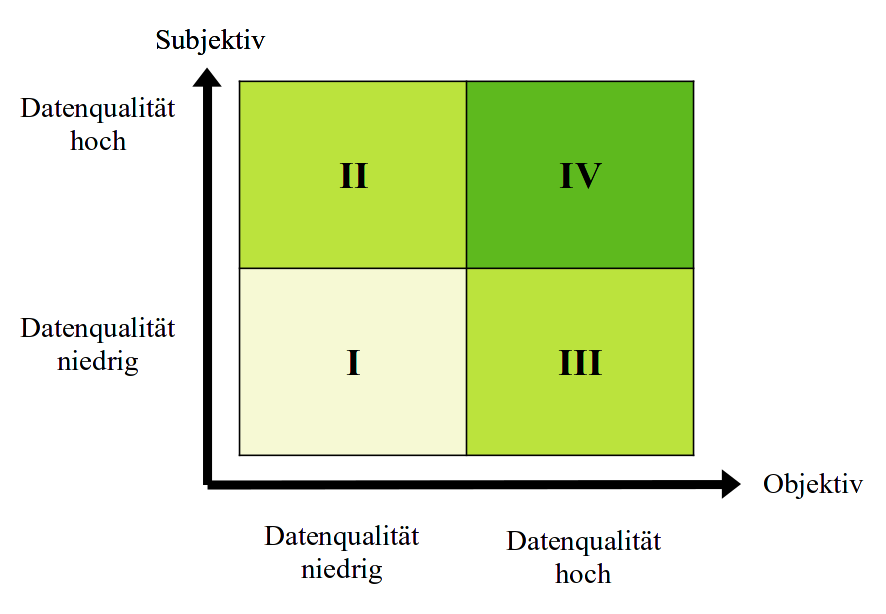
\includegraphics[width=100mm,scale=1]{content/subjektiv_objektiv.png}
\caption{Eigene Darstellung der Auswertung von objektiven und subjektiven Verfahren, basiert auf der Abbildung von \cite{pipino2002}}\label{fig:subjektiv}
\end{figure}




\section{Standardisierter Prozess}
Der Erfolg von Projekten kann durch die Verwendung eines standardisierten Prozesses deutlich gesteigert werden \cite{wirth2000}.
Einer der für Data Mining Projekte am weitesten verbreitete und eingesetzte Prozess ist der Cross Industry Standard Process for Data Mining (CRISP-DM) \cite{d.kelleher2015crispdm}.
Der Prozess beinhaltet die Phasen, die nötig sind, um ein Data Mining Projekt durchzuführen. 
Des weiteren ist definiert, welche Aufgaben in der jeweiligen Phase anfallen und welche Ergebnisse die Phasen hervorbringen \cite{wirth2000}.

\begin{figure}[h]
\centering
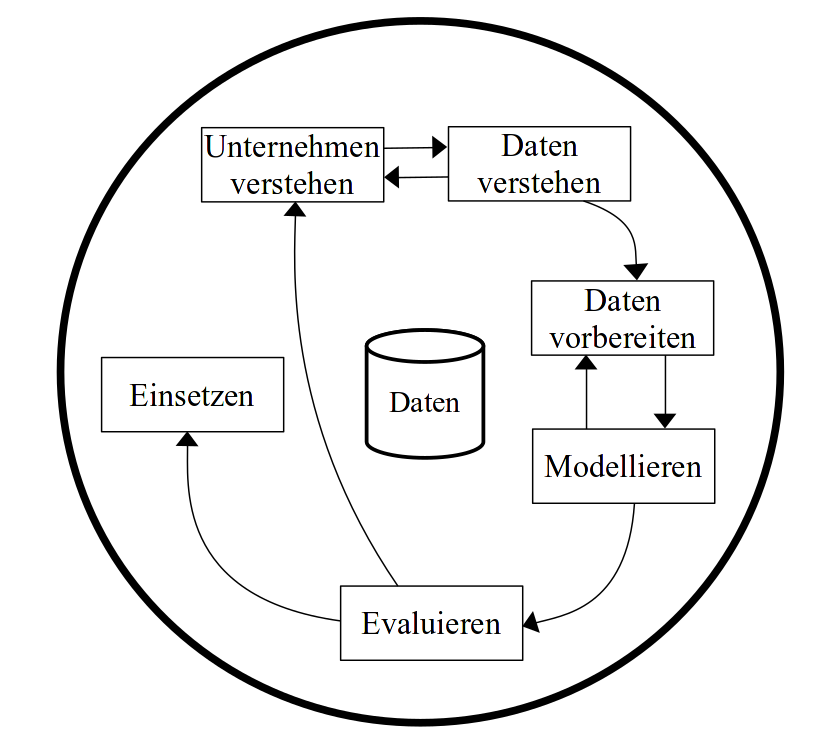
\includegraphics[width=100mm,scale=1]{content/CRISP-Prozess.png}
\caption{Eigene Darstellung des CRISP-DM, basiert auf der Abbildung von \cite{wirth2000}}\label{fig:crisp}
\end{figure}
In der \autoref{fig:crisp} sind die Phasen und ihre Ablaufreihenfolge zu sehen. 
In der Grafik ist zu erkennen, dass es sich bei dem CRISP-DM um einen iterativen Prozess handelt.
Auch in dieser Bachelorarbeit wird nach diesem Vorgehensmodell gearbeitet. 
Die Bestandteile des Modells finden sich in den einzelnen Kapiteln wieder. 
Für die Visualisierung und das Erstellen des Dashboards wird die Phase Modellieren durch Visualisieren ersetzt. 
\\

Die Bestandteile des Prozesses sind: \\
\begin{enumerate}
 \item \textbf{Unternehmen verstehen} \\
 Bei diesem Punkt ist die Aufgabe herauszufinden, welches Problem das Unternehmen versucht zu lösen \cite{d.kelleher2015crispdm}.
 
 Das Verständnis für das Problem des Unternehmens wird in dieser Bachelorarbeit in \autoref{ch:anforderungen} mit Hilfe einer Stakeholder-Analyse erlangt. Hierbei werden die betroffenen Personen untersucht und deren Wünsche aufgezeigt. Als Ergebnis werden drei mögliche Verfahren skizziert, die anschließend genauer erläutert werden.  
 
 \item \textbf{Daten verstehen} \\
 Um die Probleme mit Hilfe von Daten lösen zu können, müssen die vorhandenen Daten genau verstanden werden. Es ist wichtig zu verstehen, welche Daten in welcher Quelle vorhanden sind und um welche Datenarten es sich handelt. \cite{d.kelleher2015crispdm} 
 
 Diese Phase ist in \autoref{ch:data} umgesetzt. Dort werden die einzelnen Quellen untersucht und die Ausprägungen der Datenattribute analysiert. Des Weiteren werden in dieser Phase die für die Lösung des skizzierten Problems relevanten Daten aus den Quelltabellen ausgewählt. 
 
 \item \textbf{Daten vorbereiten} \\
 In dieser Phase wird die finale Tabelle aus den Quellen konstruiert, die zum Training der ML-Modelle verwendet wird. Typische Aufgaben in dieser Phase sind die Attributauswahl, Datenbereinigung und das Erzeugen von neuen Eigenschaften anhand der bestehenden Daten. \cite{wirth2000} Diese Tabelle wird auch als Analytical Base Table (ABT) bezeichnet \cite{d.kelleher2015crispdm}.
 
 Die Datenvorbereitung geschieht an zwei Stellen in dieser Bachelorarbeit. 
 Die Konstruktion der ABT geschieht in dem \autoref{ch:data} und die Datenbereinigung wird im \autoref{ch:experiments} durchgeführt. %TODO Lieber auch in dem Kapitel Daten mitmachen? 
 
 \item \textbf{Modellieren} \\
 In dieser Phase werden verschiedene ML-Modelle ausgewählt und getestet.
 Die Modellierungsphase ist stark verbunden mit der Datenvorbereitung, da sich einige Probleme in den Daten erst erkennen lassen, wenn die Modelle angewendet werden. 
 Auch neue Ideen für die Konstruktion von Merkmalen anhand der bestehenden Daten können in dieser Phase gefunden werden. \cite{wirth2000}
 
 Modellierung und Tests verschiedener Ansätze ist in dem \autoref{sub:machine_learning} zu sehen. 
 Zur Umsetzung der Visualisierung wird an dieser Stelle kein Modell ausgewählt und getestet, sondern die verschiedenen Data Quality Dashboard Tools untersucht. 
 Des Weiteren wird in dieser Phase die Visualisierungen in dem evaluierten Tool erzeugt und die Ergebnisse präsentiert. 
 
 \item \textbf{Evaluieren} \\
 An dieser Stelle im Prozess wird nochmals überprüft, ob das Modell die Probleme, die in Phase 1 analysiert wurden, behebt.
 Das Hauptziel ist herauszufinden, ob ein Unternehmensziel nicht gut genug durchdacht wurde. \cite{wirth2000}
 Es wird außerdem evaluiert, ob das trainierte Modell für den Einsatzzweck geeignet ist und nicht von Over- bzw. Underfitting geprägt ist. \cite{d.kelleher2015crispdm}
 
 Die Evaluation der Machine Learning Modelle erfolgt in \autoref{sub:evaluation}. 
 Dort werden die üblichen Metriken verwendet, um die Modelle zu testen und miteinander zu vergleichen. 
 
 Zur Auswertung der Visualisierung werden die gestellten Anforderungen, die in der Stakeholder-Analyse erhoben werden, mit den Ergebnissen verglichen. 
 Dies erfolgt in \autoref{sub:visualisierung}.
 
 \item \textbf{Einsetzen} \\
 Als Abschluss des Prozesses steht die Verwendung des Datenprojektes in einer produktiven Anwendung \cite{d.kelleher2015crispdm}.
 Hierzu zählt die Integration des Datenprojektes in das Unternehmen und dessen IT-Prozessen. 
 Oft wird dieser Part nicht mehr von dem Datenanalysten durchgeführt, sondern von dem Unternehmen selbst.
 Wichtig ist hierbei, dass die Schritte klar sind, was zu tun ist, um die Anwendung bzw. das ML-Modell nutzbar zu machen. \cite{wirth2000}
 
 
 %TODO Neues Unterkapitel in Experimente, dass die Integration grob beschreibt oder in den Aublick?
 Auch in dieser Arbeit werden die Schritte beschrieben, die nach dem Projekt nötig sind. 
 In großen Teilen werden diese auch schon implementiert und durchgeführt. 
 Lediglich das automatisierte Starten der Programme muss durch die Entwicklungsabteilung hinzugefügt werden, da diese es in ihrer Programmsteuerung hinterlegen können. 
 In diesem Projekt wird eine solche Steuerung beispielhaft mit der Verwendung von CRON-Jobs beschrieben. 
\end{enumerate}




